\documentclass[spanish]{article}

%%%%%%%%%%%%%%%%%%%%%%%%%%%%%%%%%%%%%%%%%%%%%%%%%%%%%%%%%%%%%%%%%%%%%%%%%%%%%%%%

% Language
\usepackage[spanish]{babel}

% Support for images
\usepackage{graphicx}

% Avoiding indenting of first paragraph's line.
\setlength{\parindent}{0cm}

% Support for hyperlinks.
\usepackage{hyperref}
\hypersetup {
        linktoc=all,
        hidelinks
}

% Additional section formatting.
\renewcommand\thesection{\arabic{section}}
\renewcommand\thesubsection{\thesection.\arabic{subsection}}

% Cover of the document
\title{Sistemas Operativos - Práctica 1}
\author{Oussama Akachach Jouhrati\\[0.5cm]{\small Profesor/a: Montserrat Ferrer
Serafí}}
\date{\today}

%%%%%%%%%%%%%%%%%%%%%%%%%%%%%%%%%%%%%%%%%%%%%%%%%%%%%%%%%%%%%%%%%%%%%%%%%%%%%%%%

\begin{document}

\pagenumbering{gobble}
\maketitle
\newpage

\tableofcontents
\pagenumbering{arabic}
\setcounter{page}{2}
\newpage

% Customize from here.

\section{Ejercicio 1}

\subsection{Apartado 1.1}

\subsubsection{Apartado 1.1.1}

\begin{center}
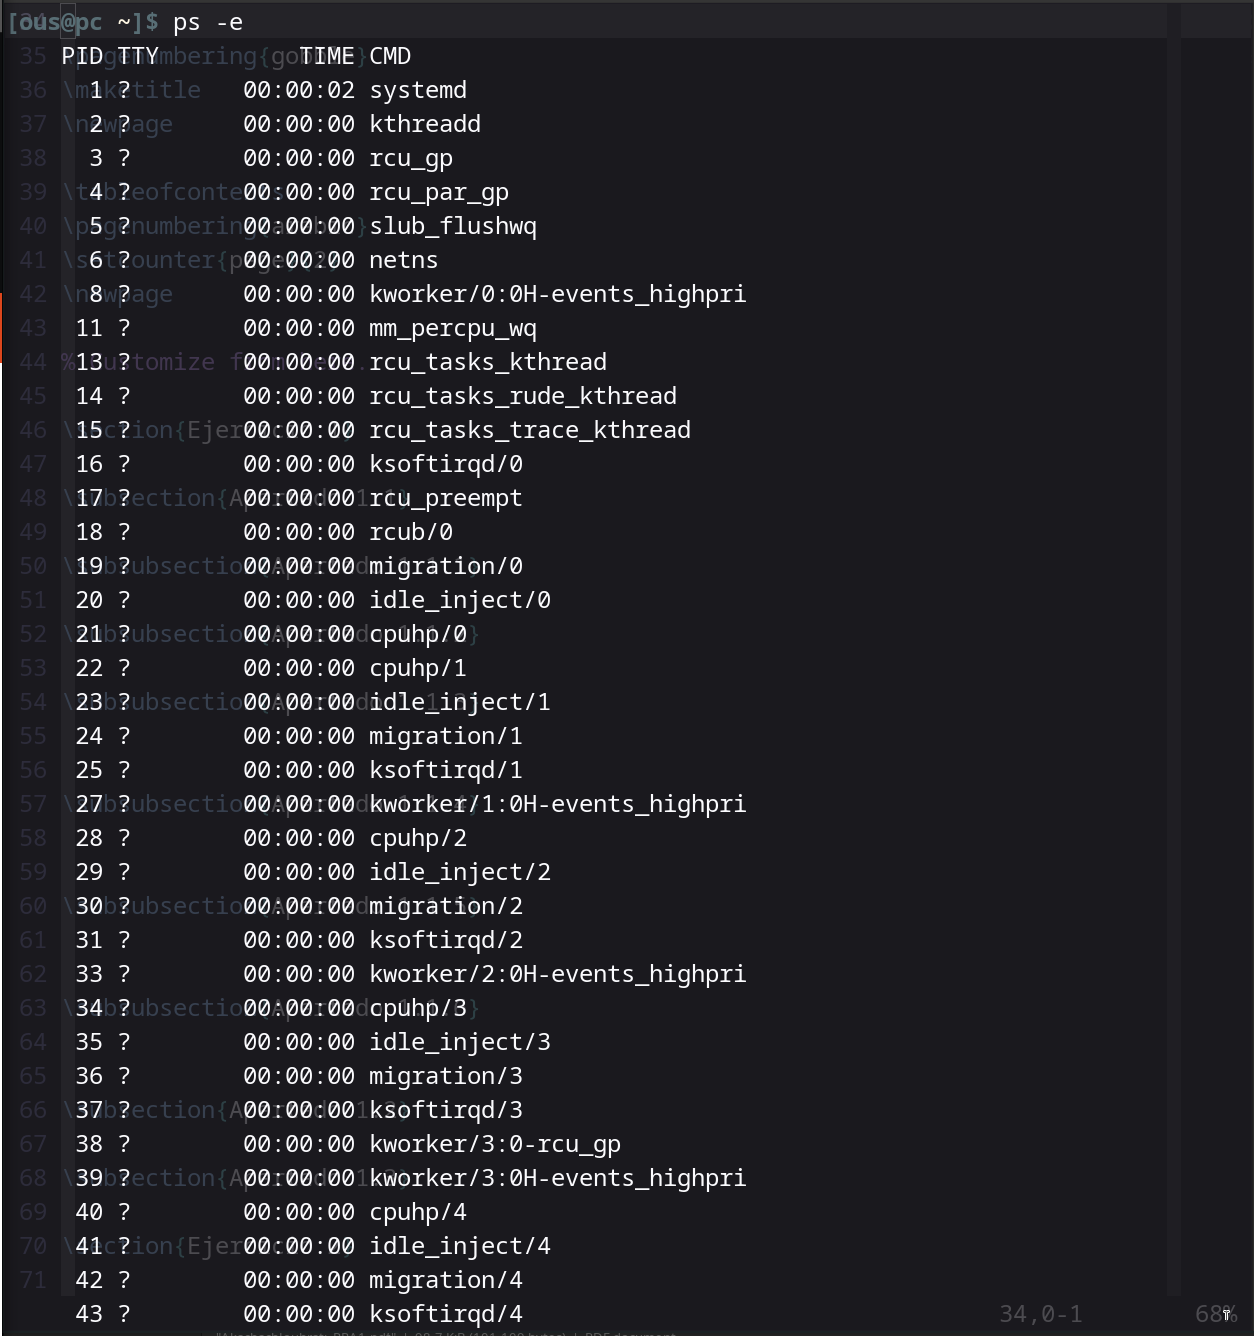
\includegraphics[scale=.3]{../img/1.png}
\end{center}

\newpage

\subsubsection{Apartado 1.1.2}

\begin{center}
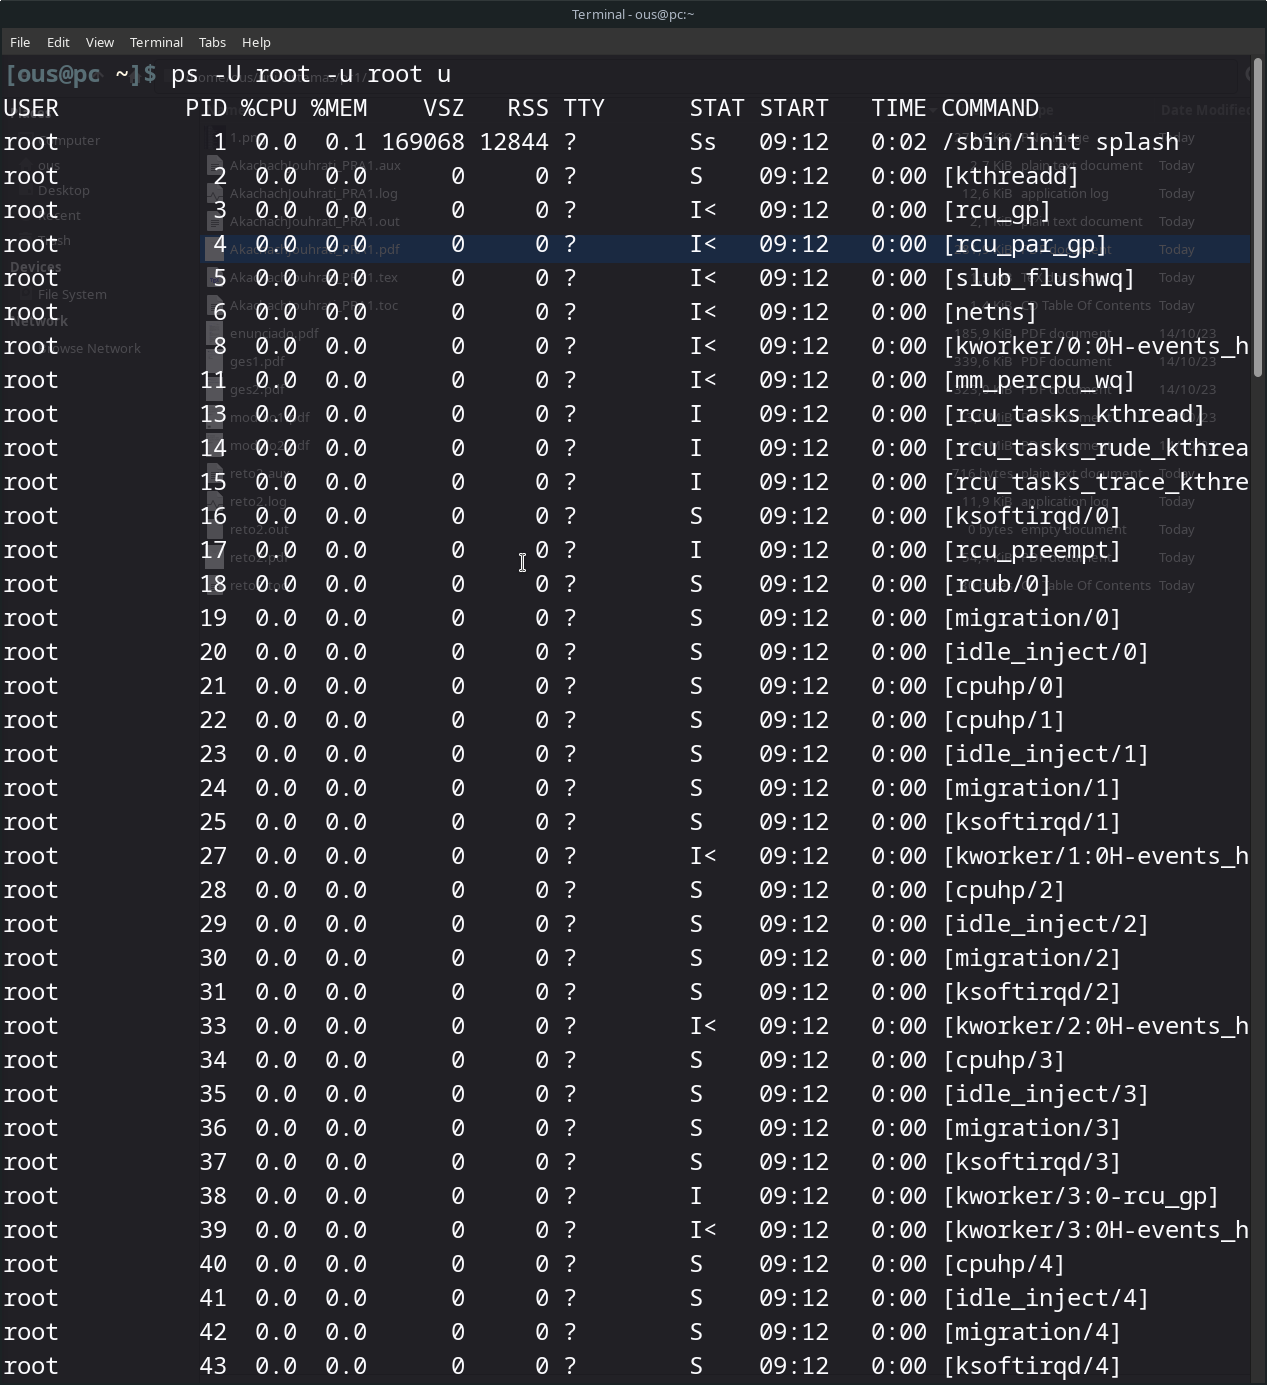
\includegraphics[scale=.3]{../img/2.png}
\end{center}

\newpage

\subsubsection{Apartado 1.1.3}

\begin{center}
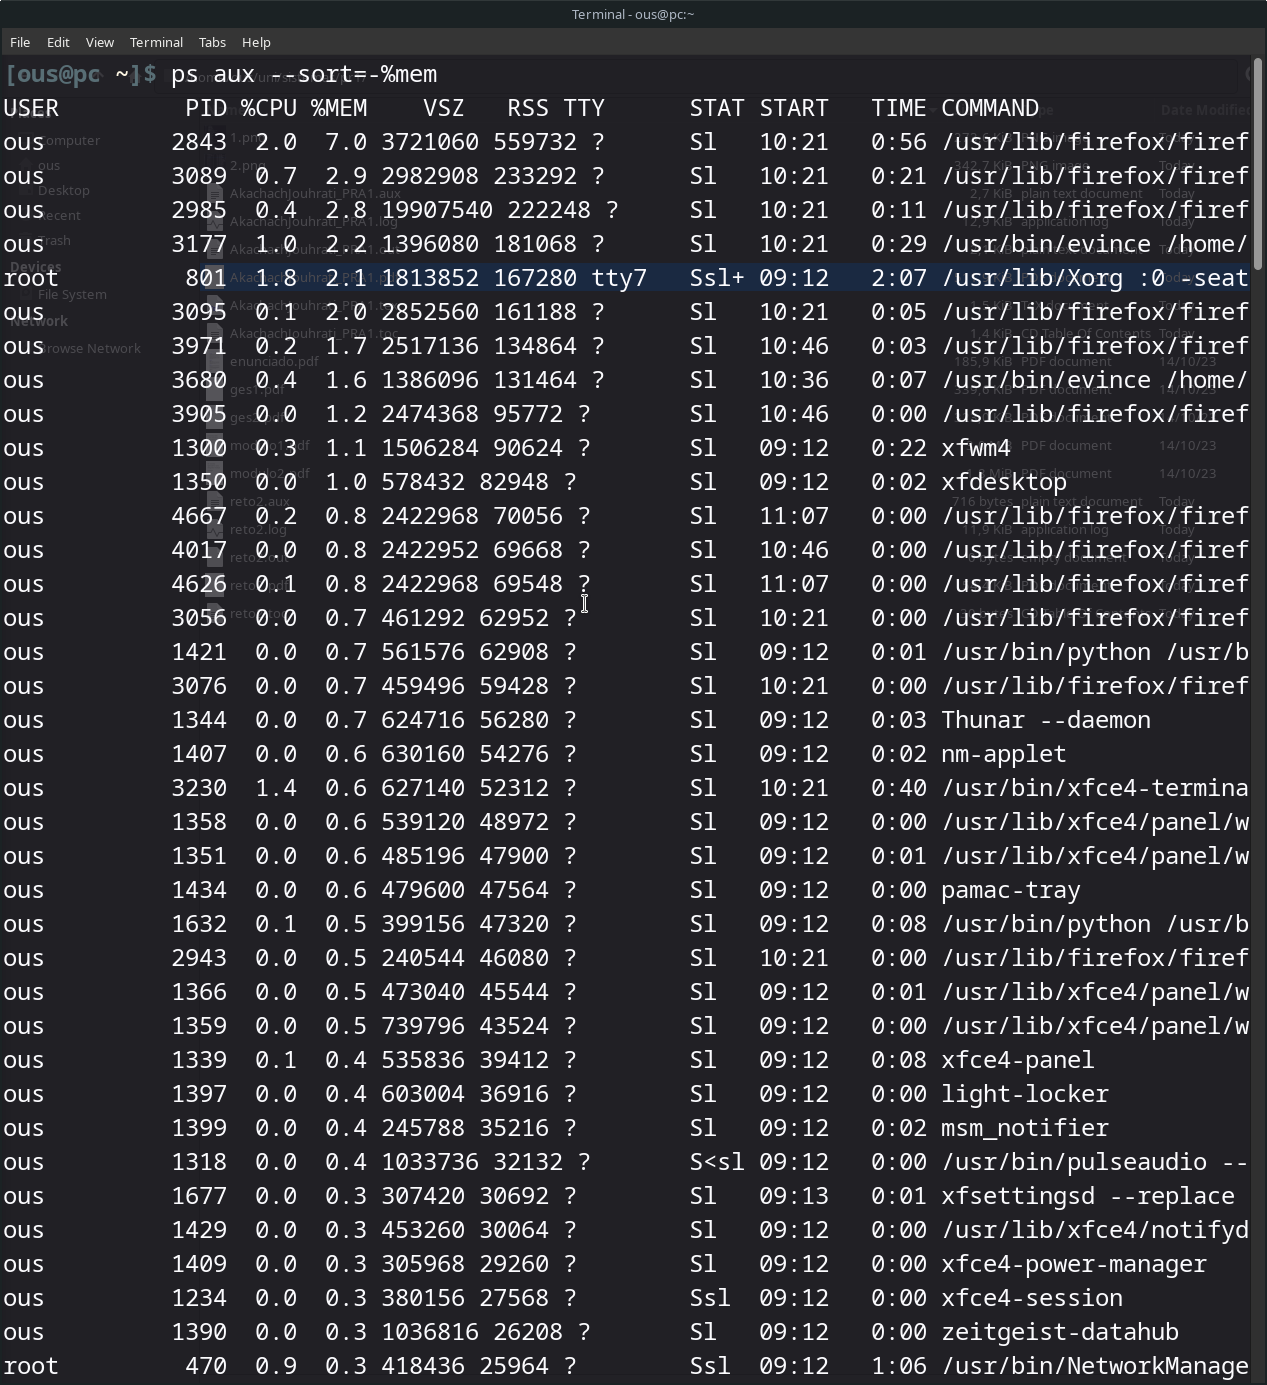
\includegraphics[scale=.3]{../img/3.png}
\end{center}

El proceso que más memoria está ocupando es Firefox, ocupando un 7\% de la
memoria actual.

\newpage

\subsubsection{Apartado 1.1.4}

\begin{center}
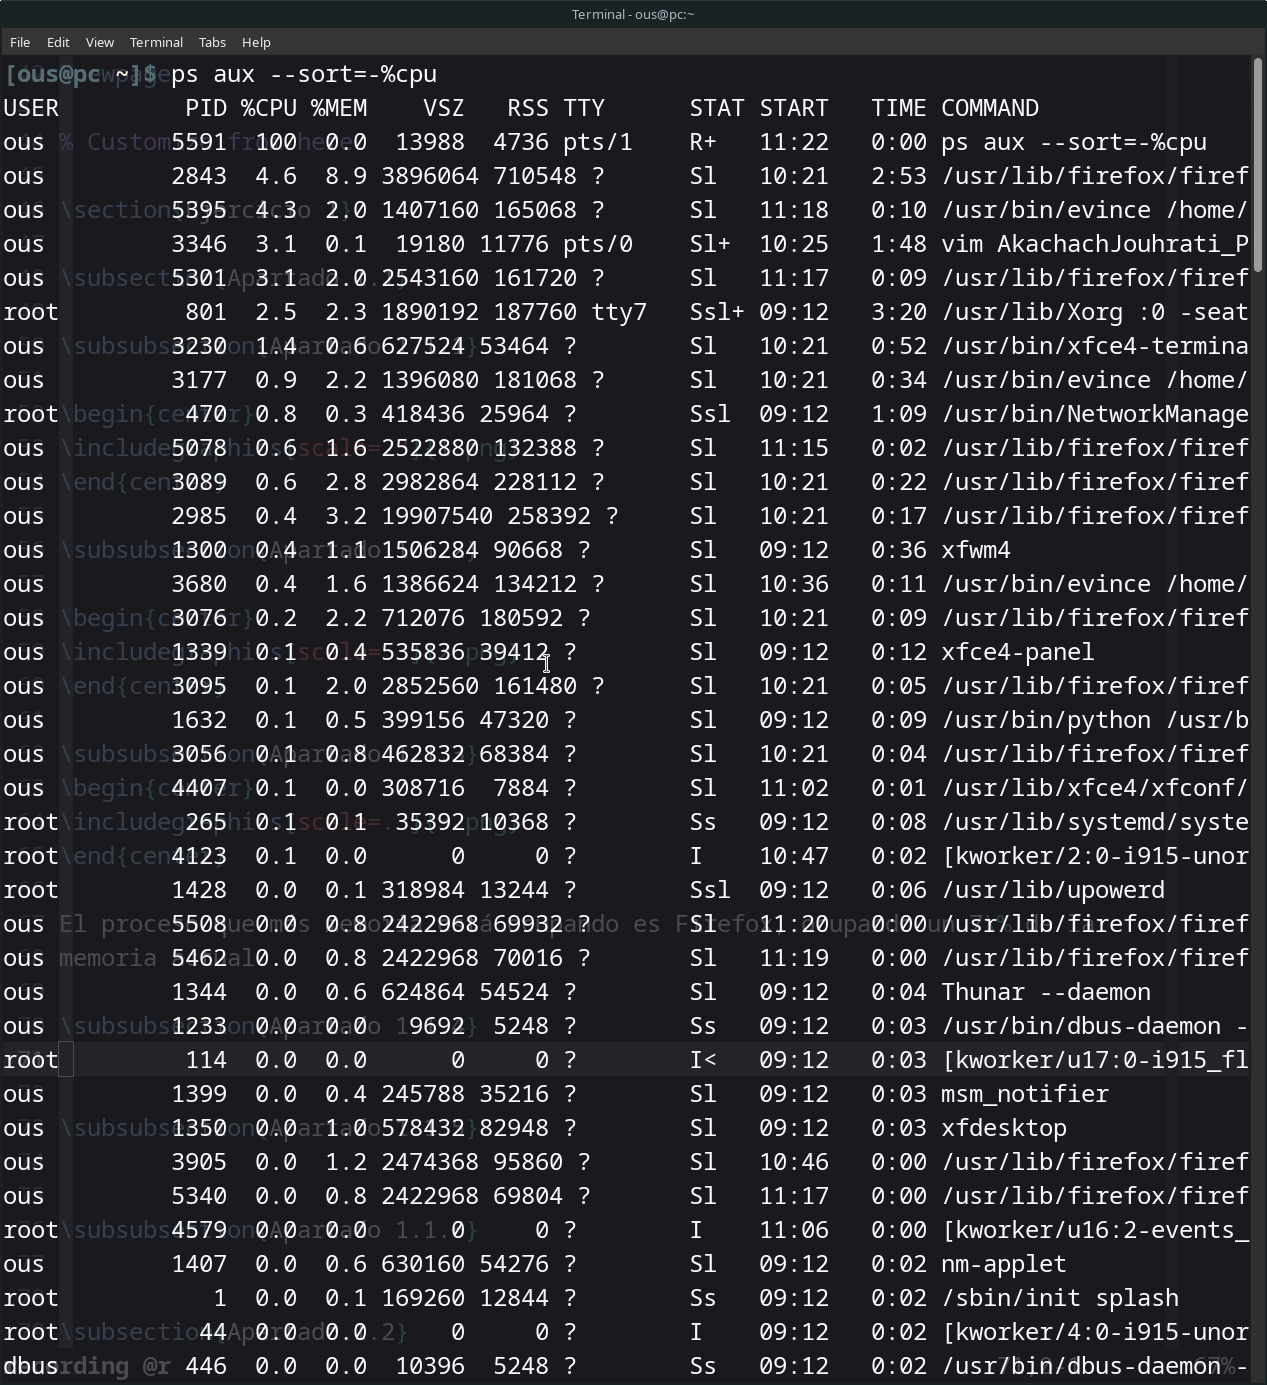
\includegraphics[scale=.3]{../img/4.png}
\end{center}

El proceso que mas espacio físico está ocupando es Firefox, ocupando un 4.6\%
del espacio lógico.

\newpage

\subsubsection{Apartado 1.1.5}

\begin{center}
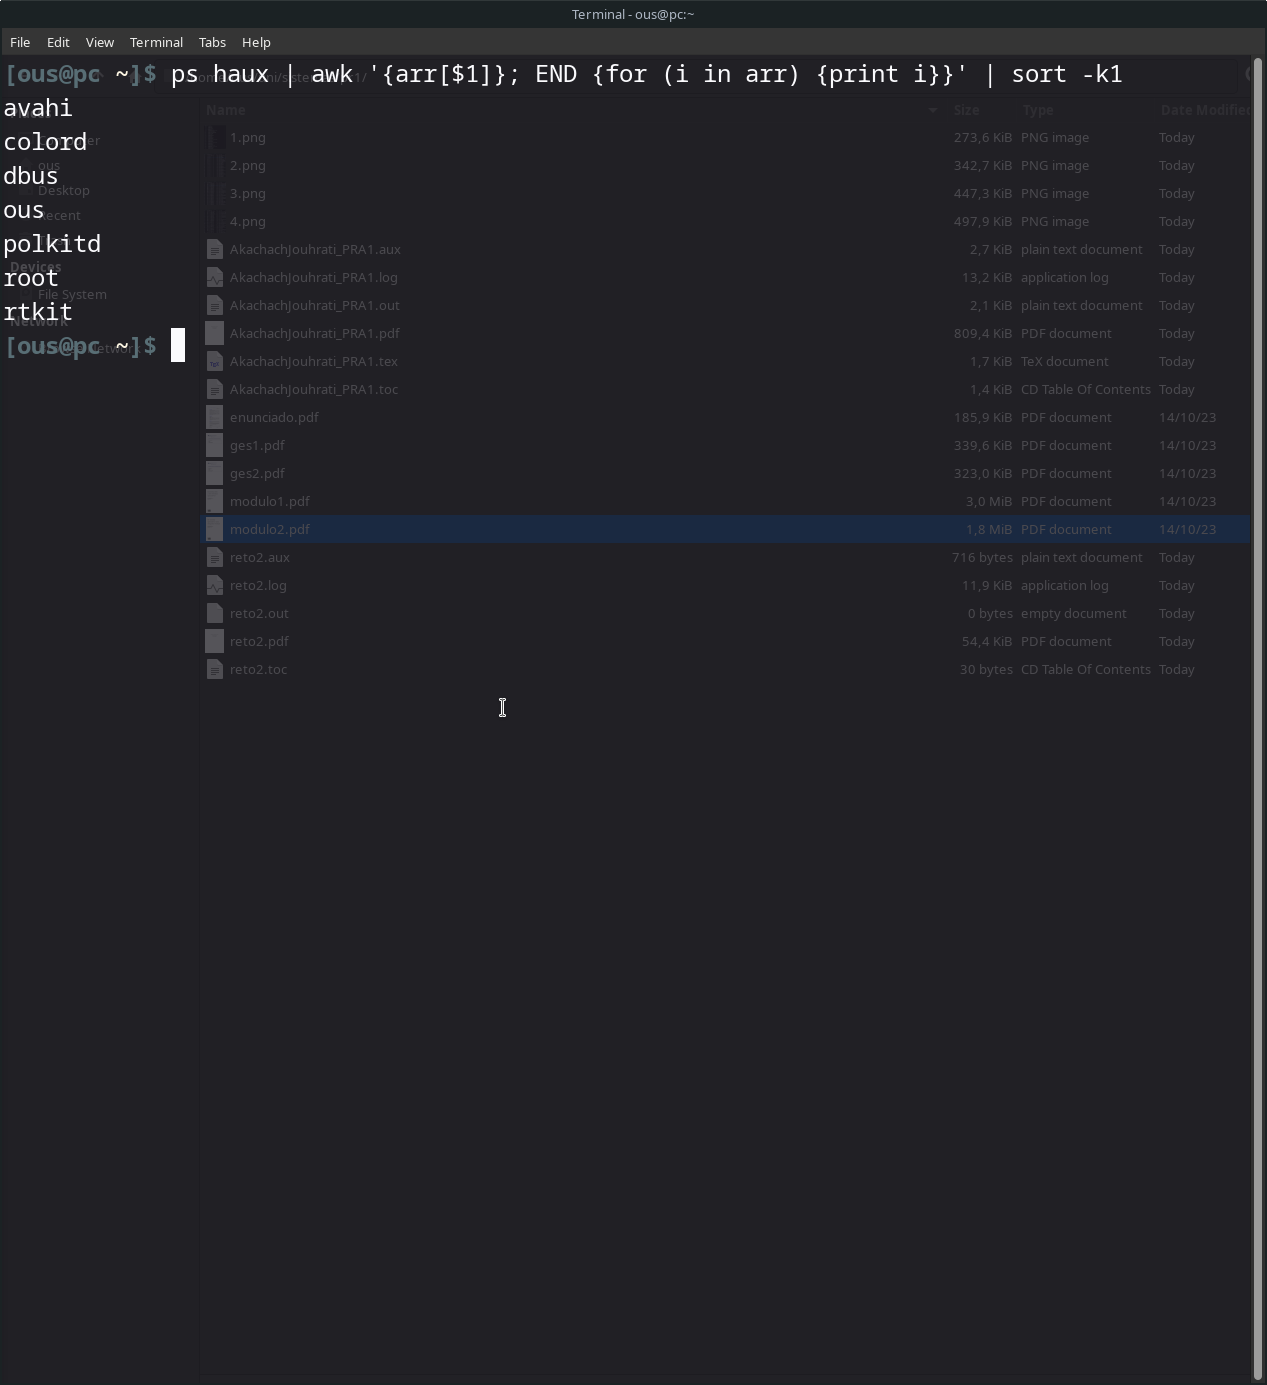
\includegraphics[scale=.3]{../img/5.png}
\end{center}

\newpage

\subsubsection{Apartado 1.1.6}

\begin{center}
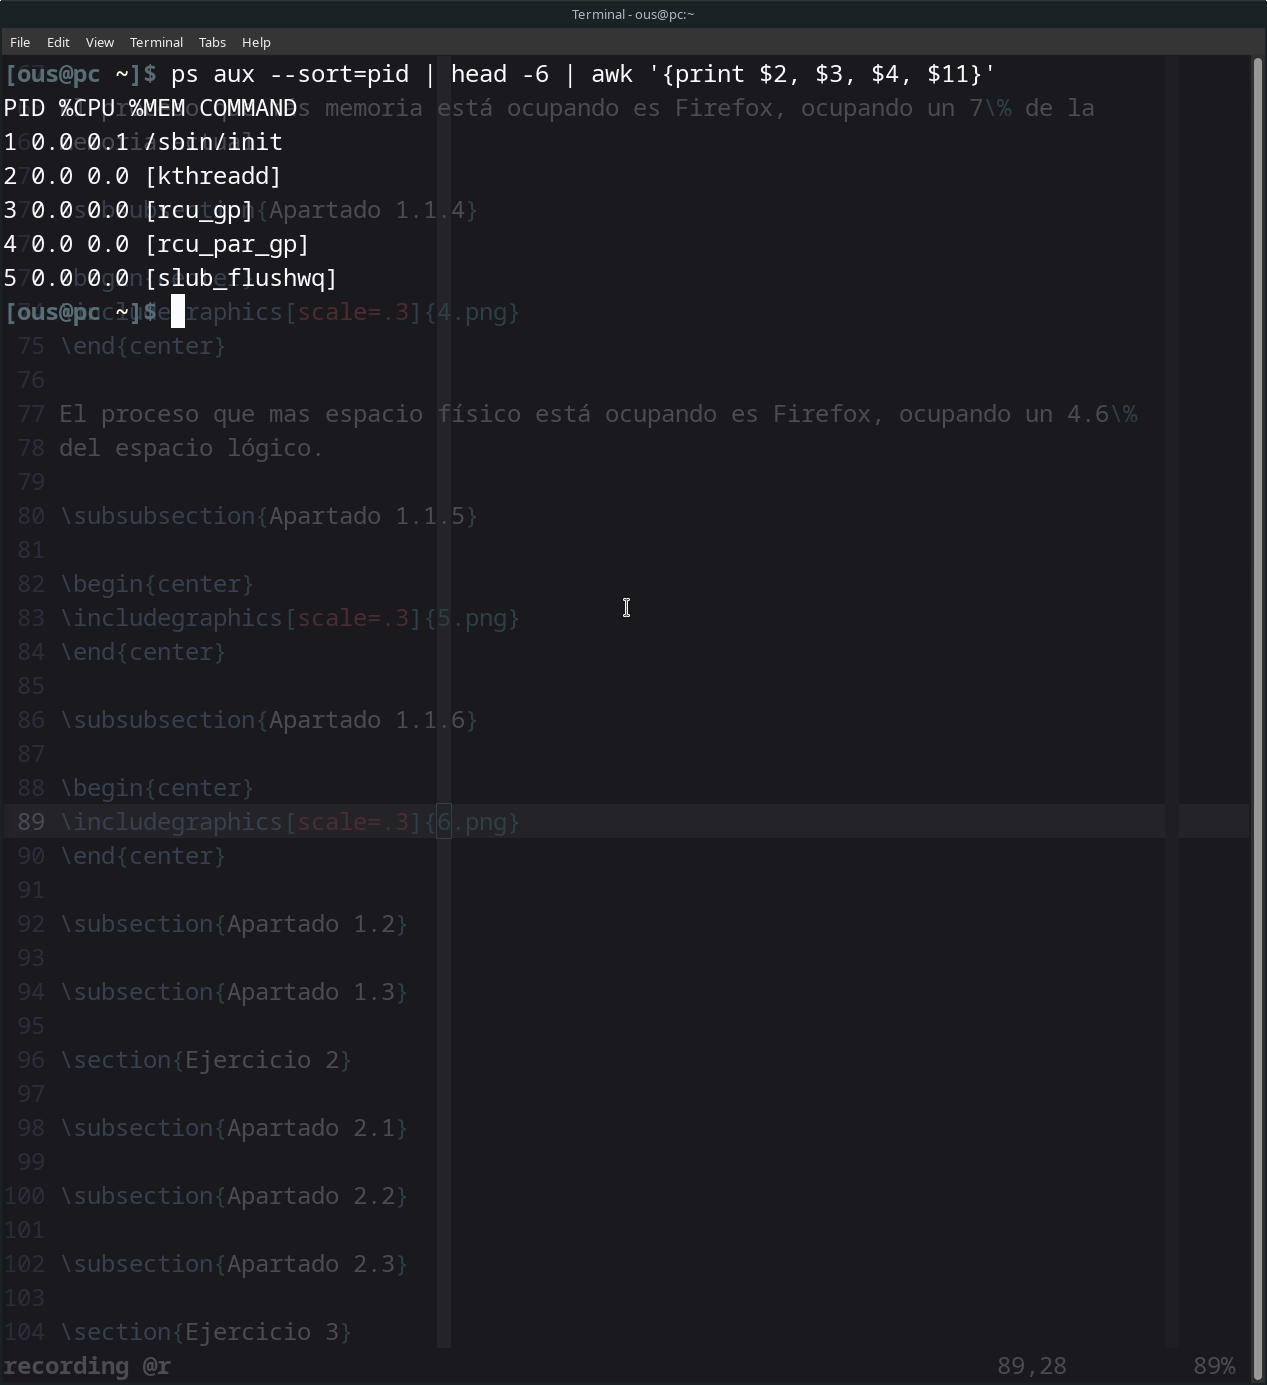
\includegraphics[scale=.3]{../img/6.png}
\end{center}

\newpage

\subsection{Apartado 1.2}

\subsubsection{Apartado 1.2.1}

Podemos saber si una instrucción de un programa es una llamada al sistema si lo
que pretende es entrar al modo kernel para acceder a un proceso. En caso de que
sea una rutina de biblioteca, la instrucción pedirá acceso a una función de la
biblioteca de un lenguaje de programación. Los modos de acceso son diferentes,
ya que en el caso de una llamada al sistema, en el modo kernel los programas
acceden directamente a los recursos de hardware y en el modo usuario, que es el
modo de las rutinas de biblioteca, estos recursos no son accesibles
directamente.

\subsubsection{Apartado 1.2.2}

Por lo general, son más rápidas, ya que no hay cambio de contexto, es decir,
pasar de modo usuario a modo kernel y viceversa. También son más portables,
porque son parte de la biblioteca de tu lenguaje de programación, y no parten
del kernel, en cuestión.

\subsubsection{Apartado 1.2.3}

\textit{Podemos encontrar la solución a este apartado en el archivo suma1.c.}

\subsection{Apartado 1.3}

\textit{Podemos encontrar la solución a este apartado en el archivo suma2.c.}

\newpage

\section{Ejercicio 2}

\subsection{Apartado 2.1}

La principal diferencia entre utilizar memoria estática y utilizar una
asignación dinámica de memoria es que la primera está definida de manera fija,
antes de la ejecución del programa, mientras que en la segunda, la cantidad de
memoria necesaria está definida de manera variable y se define durante la
ejecución del programa. Dicho de otra manera, en la asignación estática de
memoria, esta se asigna en el tiempo de compilación y, en el caso de la
asignación dinámica de memoria, esta se asigna en el tiempo de ejecución o
runtime.\newline

La asignación estática de memoria es menos eficiente que la dinámica, puesto que
con la dinámica podemos utilizar exactamente la cantidad necesaria para cumplir
nuestro objetivo deseado, mientras que de la otra manera reservamos una cantidad
de memoria que nos puede ser útil, o no, para nuestro programa.\newline

Como en la asignación dinámica de memoria, esta varía durante la ejecución del
programa, la podemos reutilizar en el mismo, mientras que en la asignación de
memoria estática, no podemos hacer esto, puesto que está ocupada hasta el fin de
la ejecución de este.\newline

\newpage

\subsection{Apartado 2.2}

\subsubsection{Apartado 2.2.1}

\begin{center}
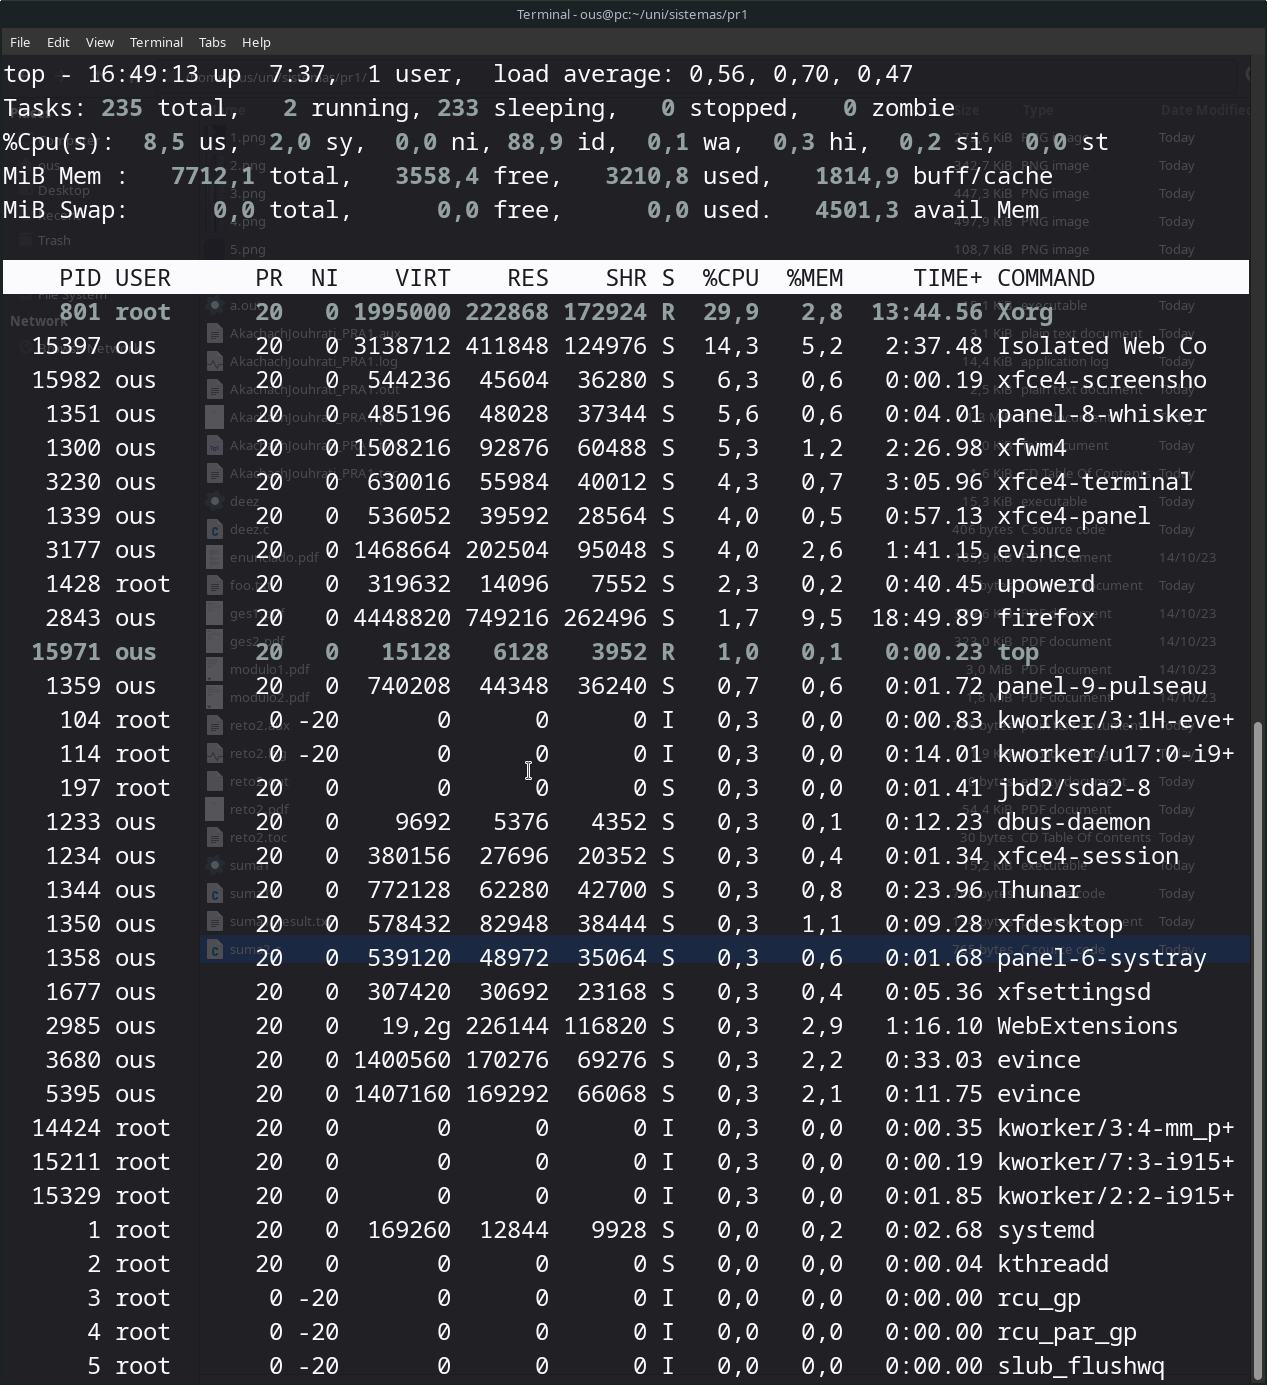
\includegraphics[scale=.3]{../img/7.png}
\end{center}

\newpage

\subsubsection{Apartado 2.2.2}

\begin{center}
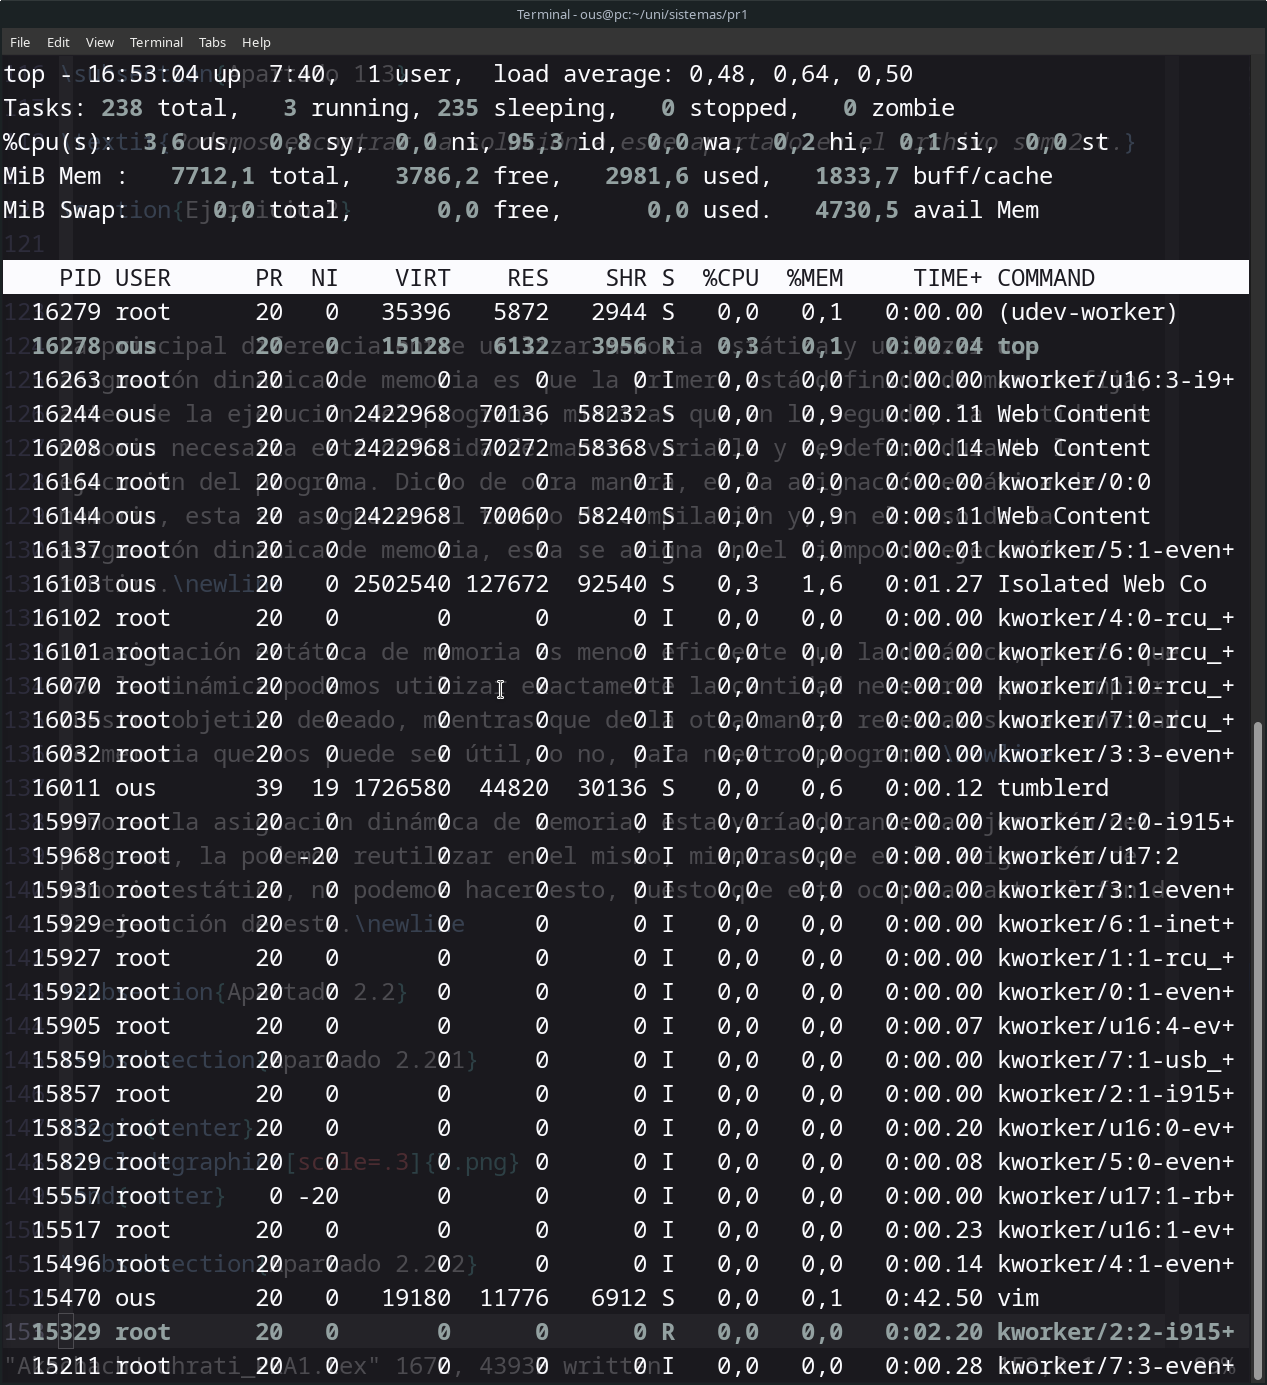
\includegraphics[scale=.25]{../img/8.png}
\end{center}

Para cambiar el orden, añadimos la opción -o, seguido del sentido (+ para
hacerlo de mayor a menor, - para hacerlo de menor a mayor), junto con el nombre
del campo el cual queremos ordenar.\newline

Para ordenar los procesos en top por PID de mayor a menor, debemos introducir el
siguiente comando:\newline

\begin{center}
\textbf{top -o +PID}
\end{center}

\newpage

\subsubsection{Apartado 2.2.3}

VIRT es la cantidad de memoria virtual que utiliza un proceso.\newline

RES es la cantidad de memoria física que utiliza un proceso.\newline

\%MEM es el porcentaje de memoria utilizado por un proceso, del total. Se trata
del cuociente de RES por el total de memoria física.

\subsection{Apartado 2.3}

\begin{center}
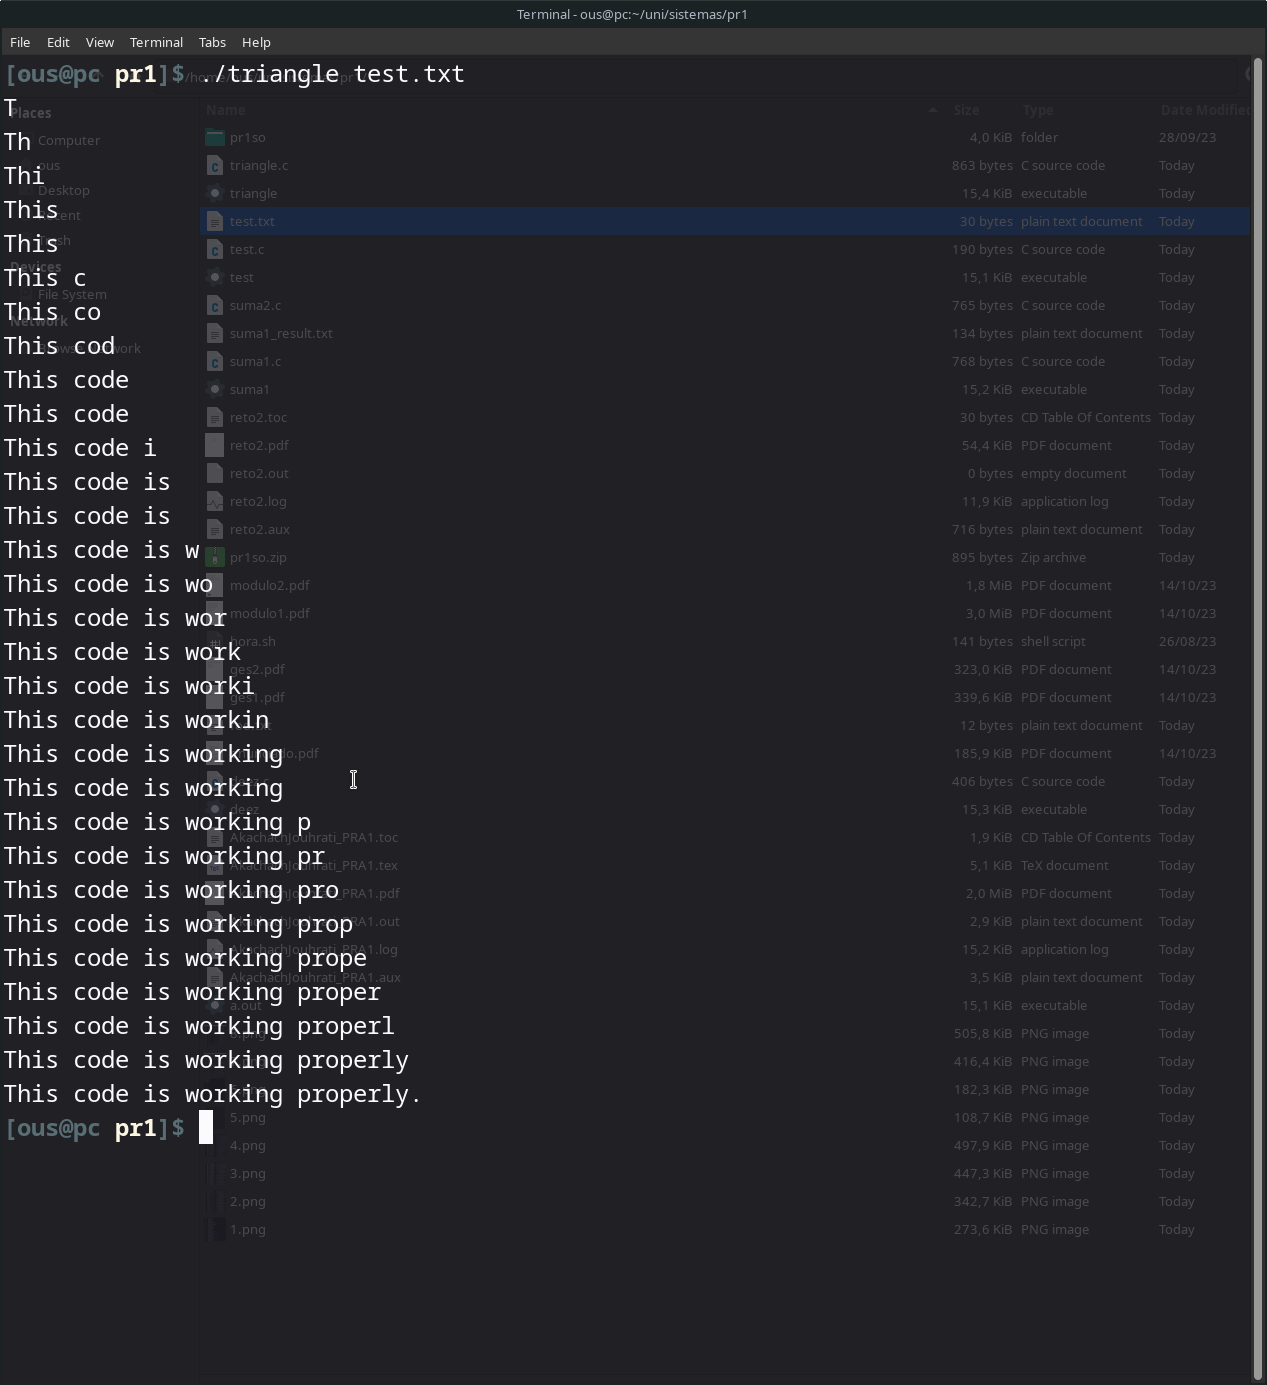
\includegraphics[scale=.25]{../img/9.png}
\end{center}

\textit{Podemos encontrar la solución a este apartado en el archivo triangle.c.}

\newpage

\section{Ejercicio 3}

\subsection{Apartado 3.1}

\subsubsection{Apartado 3.1.1}

\begin{center}
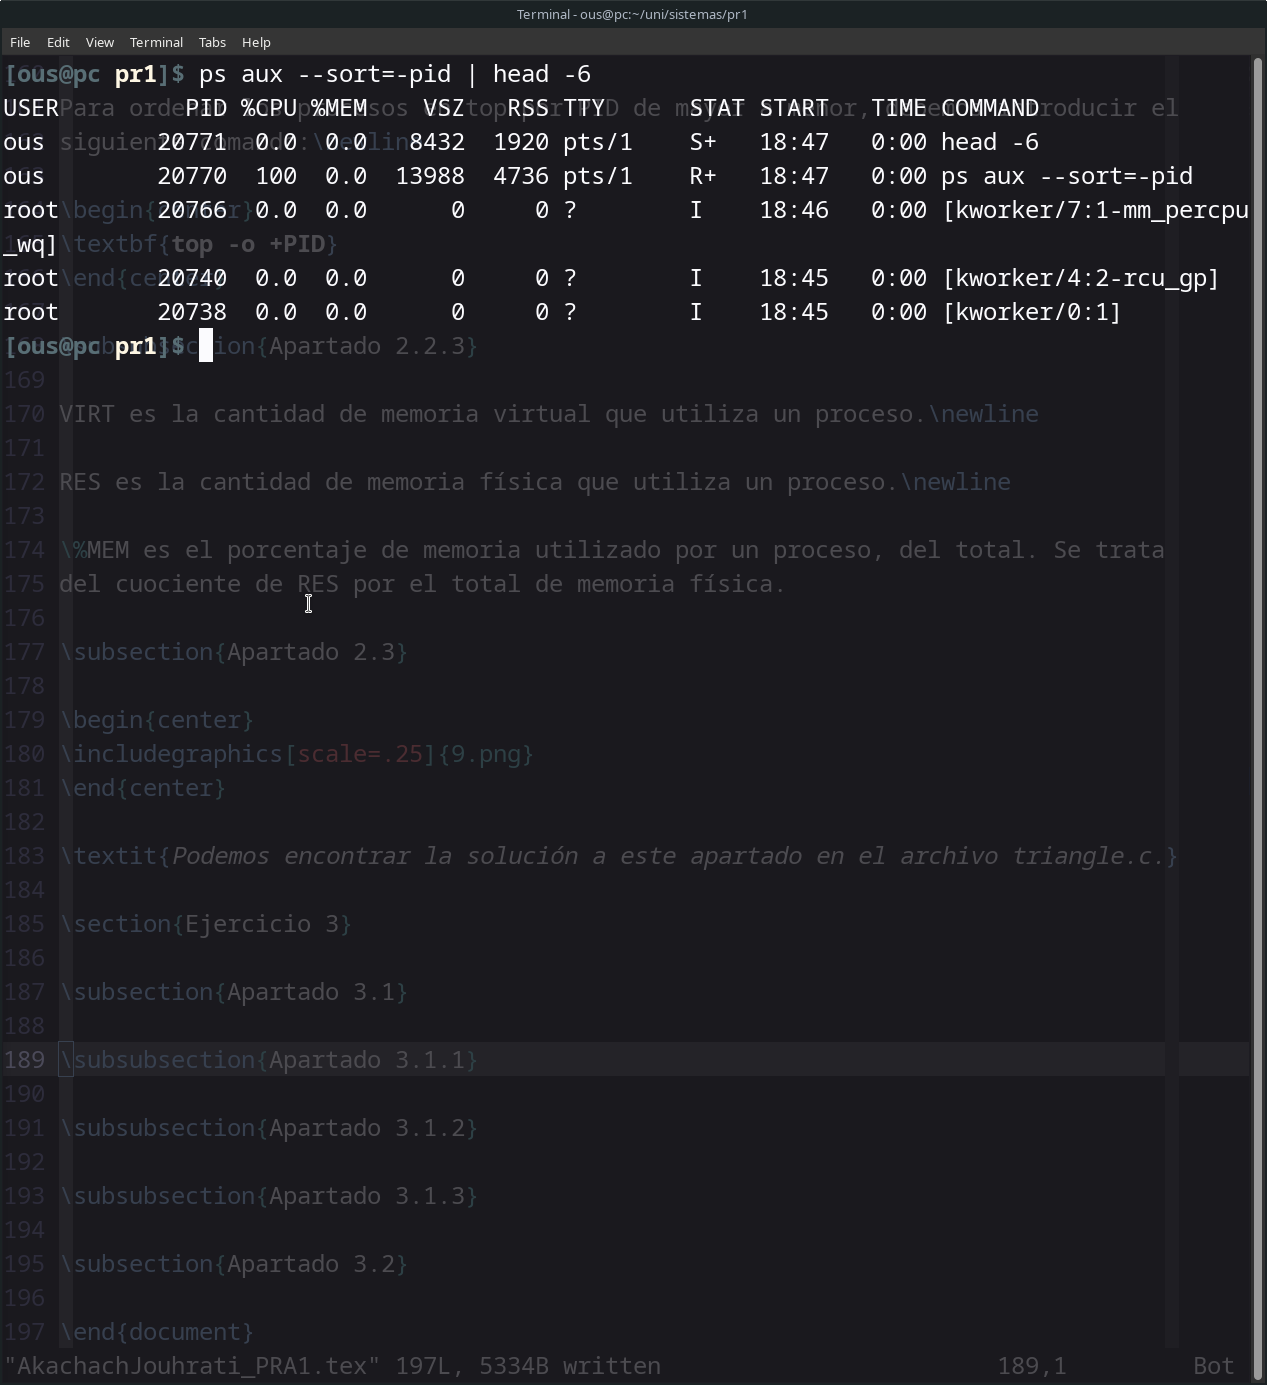
\includegraphics[scale=.25]{../img/10.png}
\end{center}

\newpage

\subsubsection{Apartado 3.1.2}

\begin{center}
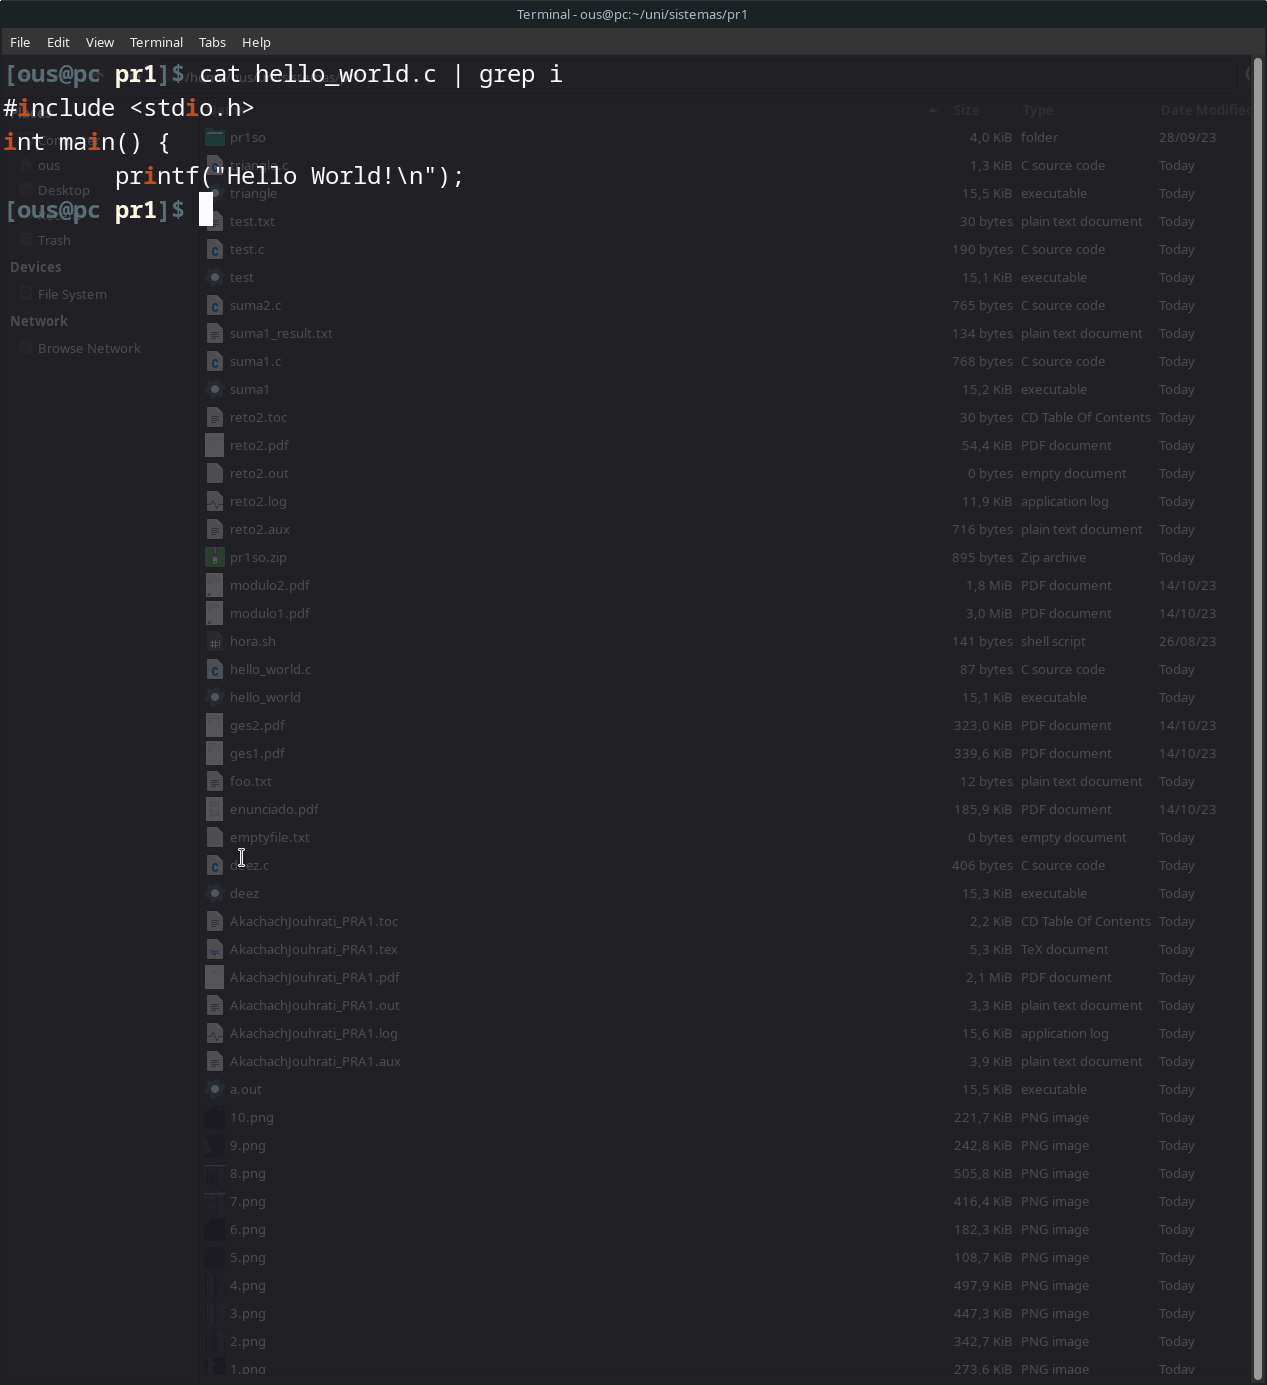
\includegraphics[scale=.25]{../img/11.png}
\end{center}

\newpage

\subsubsection{Apartado 3.1.3}

\begin{center}
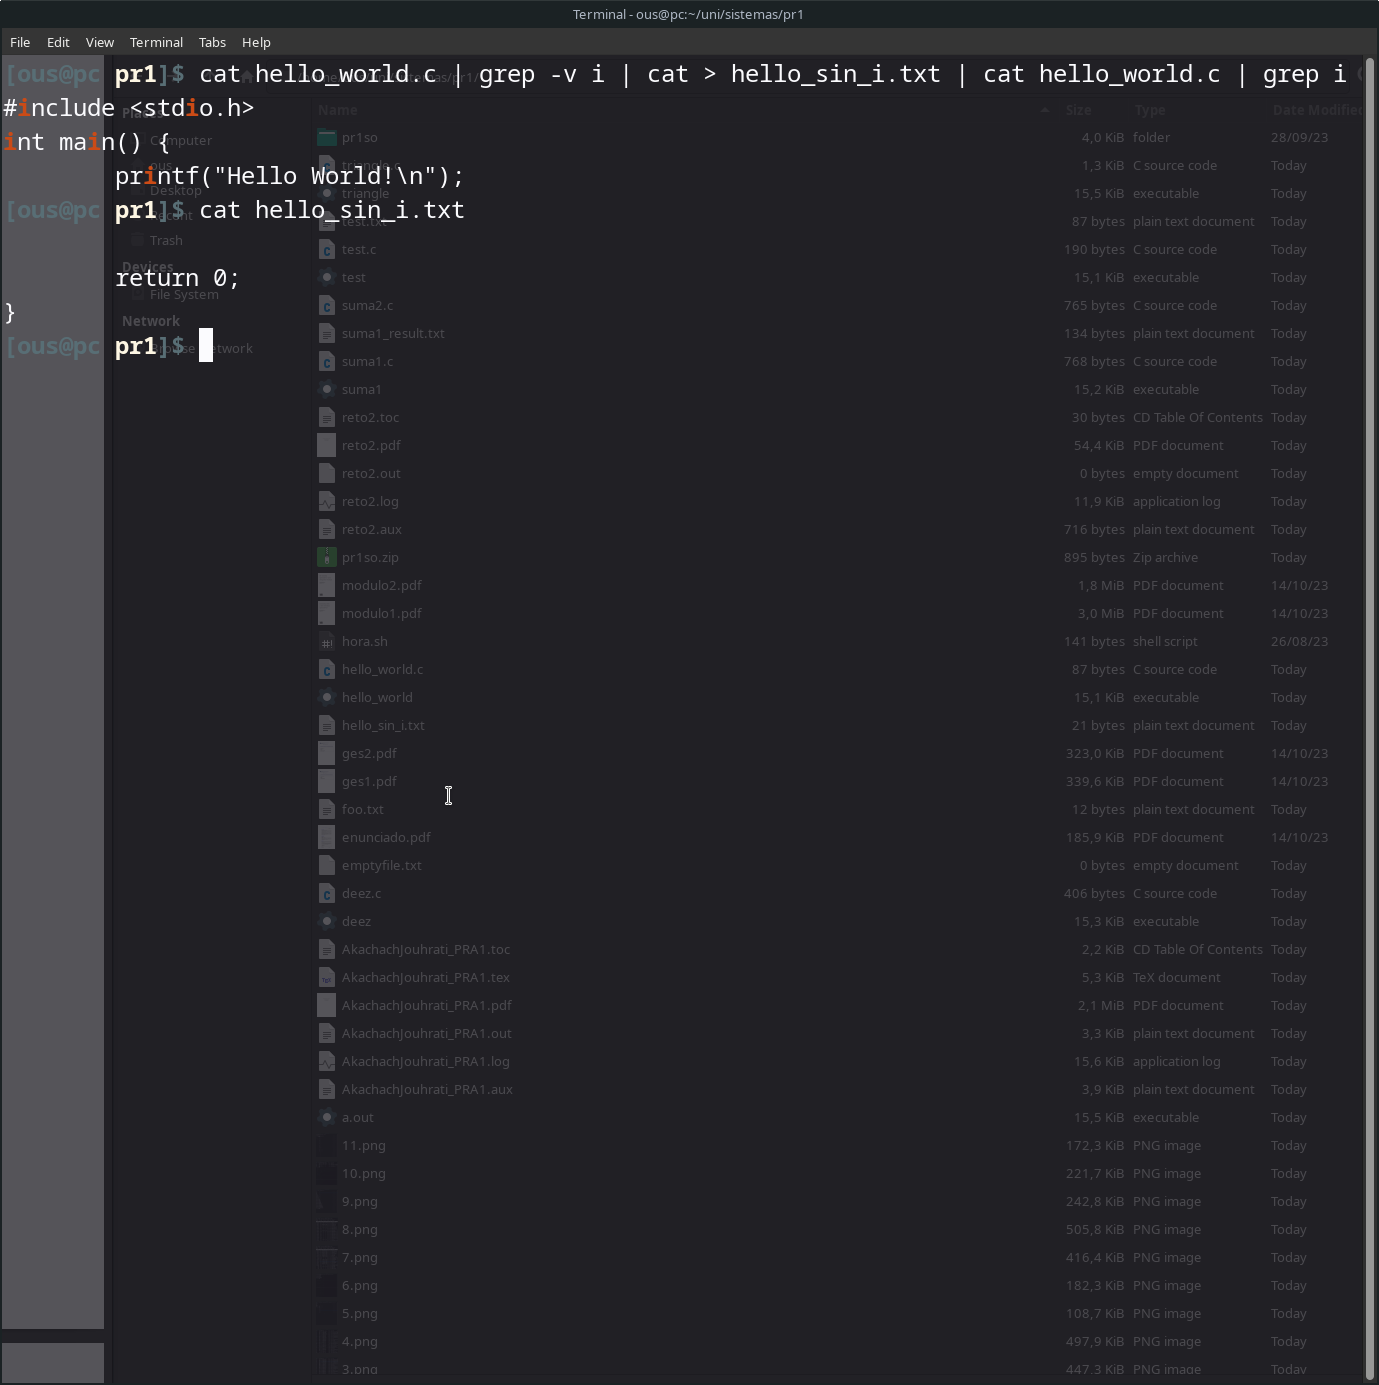
\includegraphics[scale=.25]{../img/12.png}
\end{center}

\newpage

\subsection{Apartado 3.2}

\subsubsection{Apartado 3.2.1}

\begin{center}
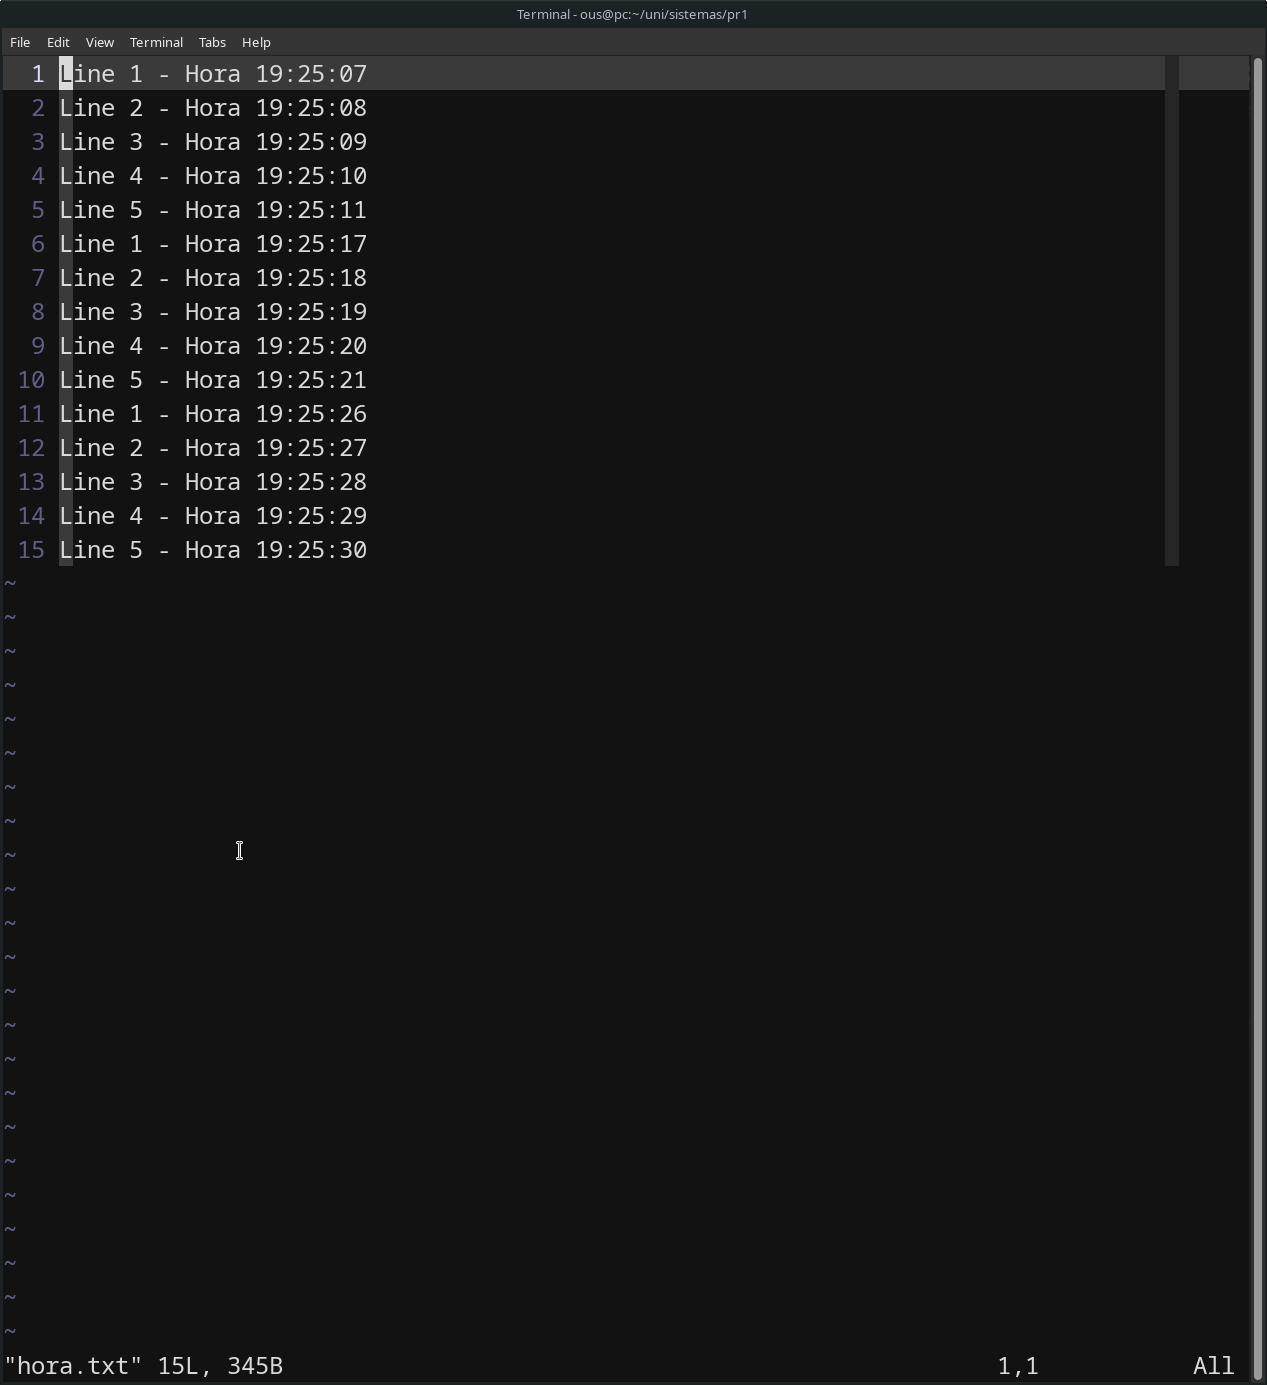
\includegraphics[scale=.25]{../img/13.png}
\end{center}

\newpage

\subsubsection{Apartado 3.2.2}

\begin{center}
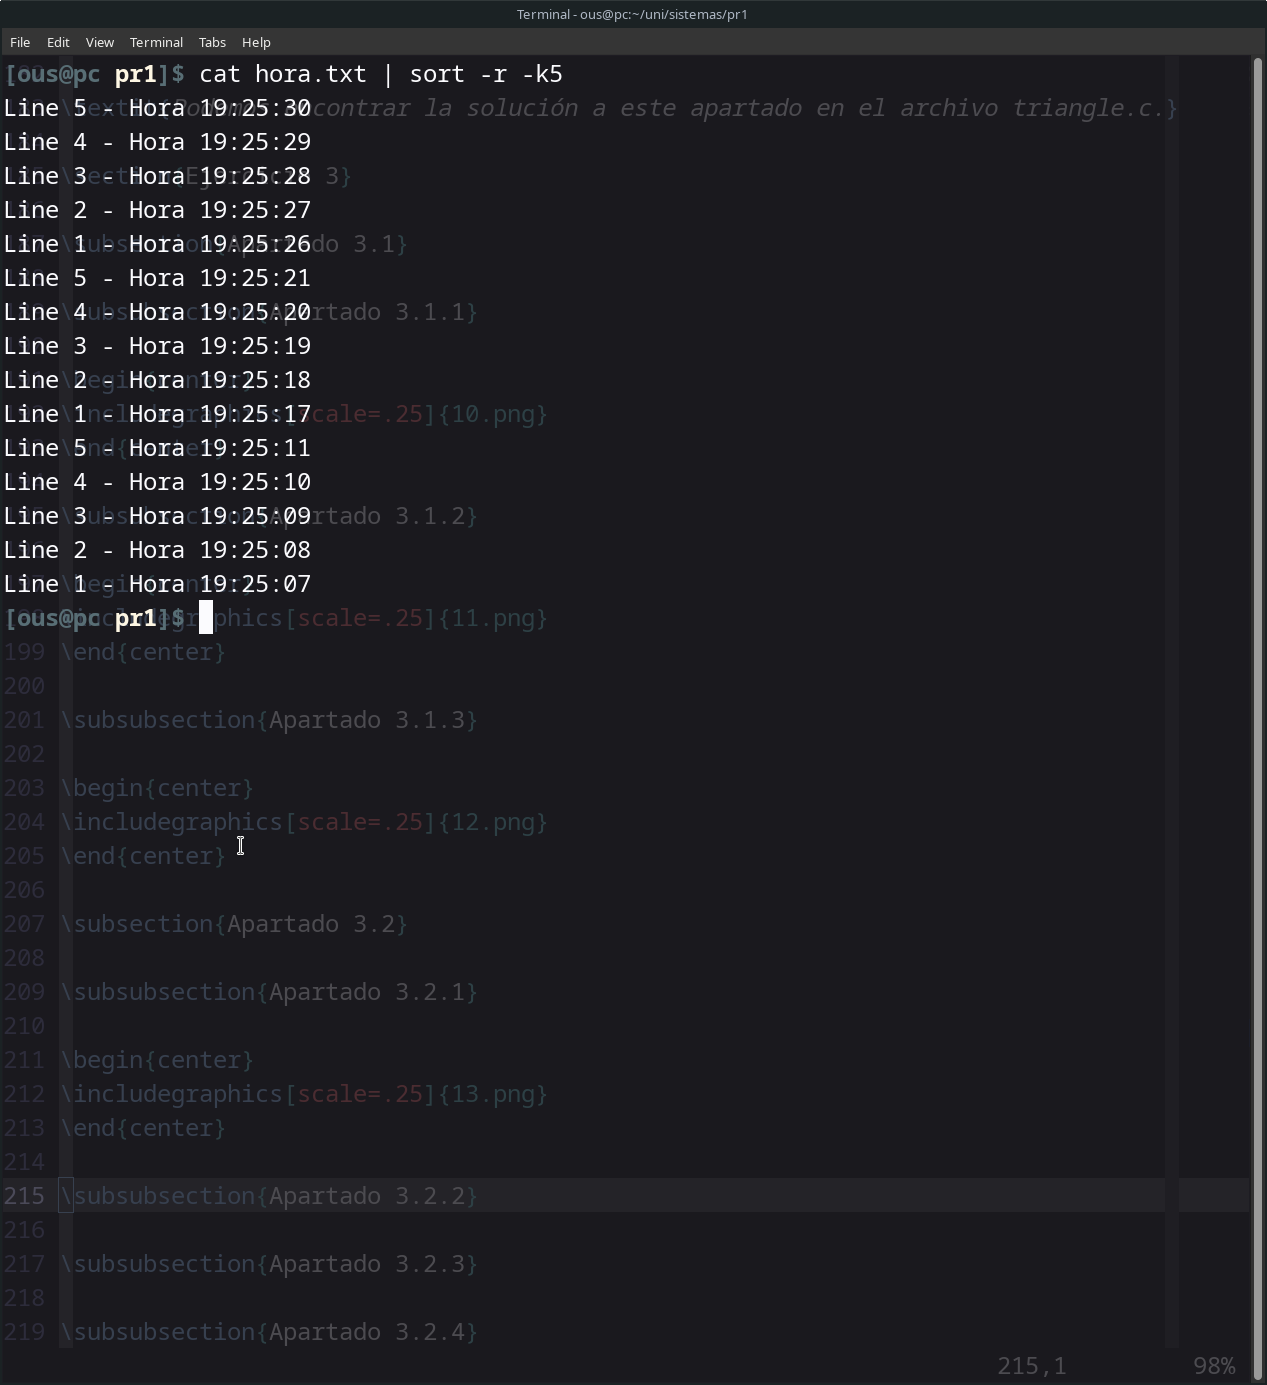
\includegraphics[scale=.25]{../img/14.png}
\end{center}

\newpage

\subsubsection{Apartado 3.2.3}

\begin{center}
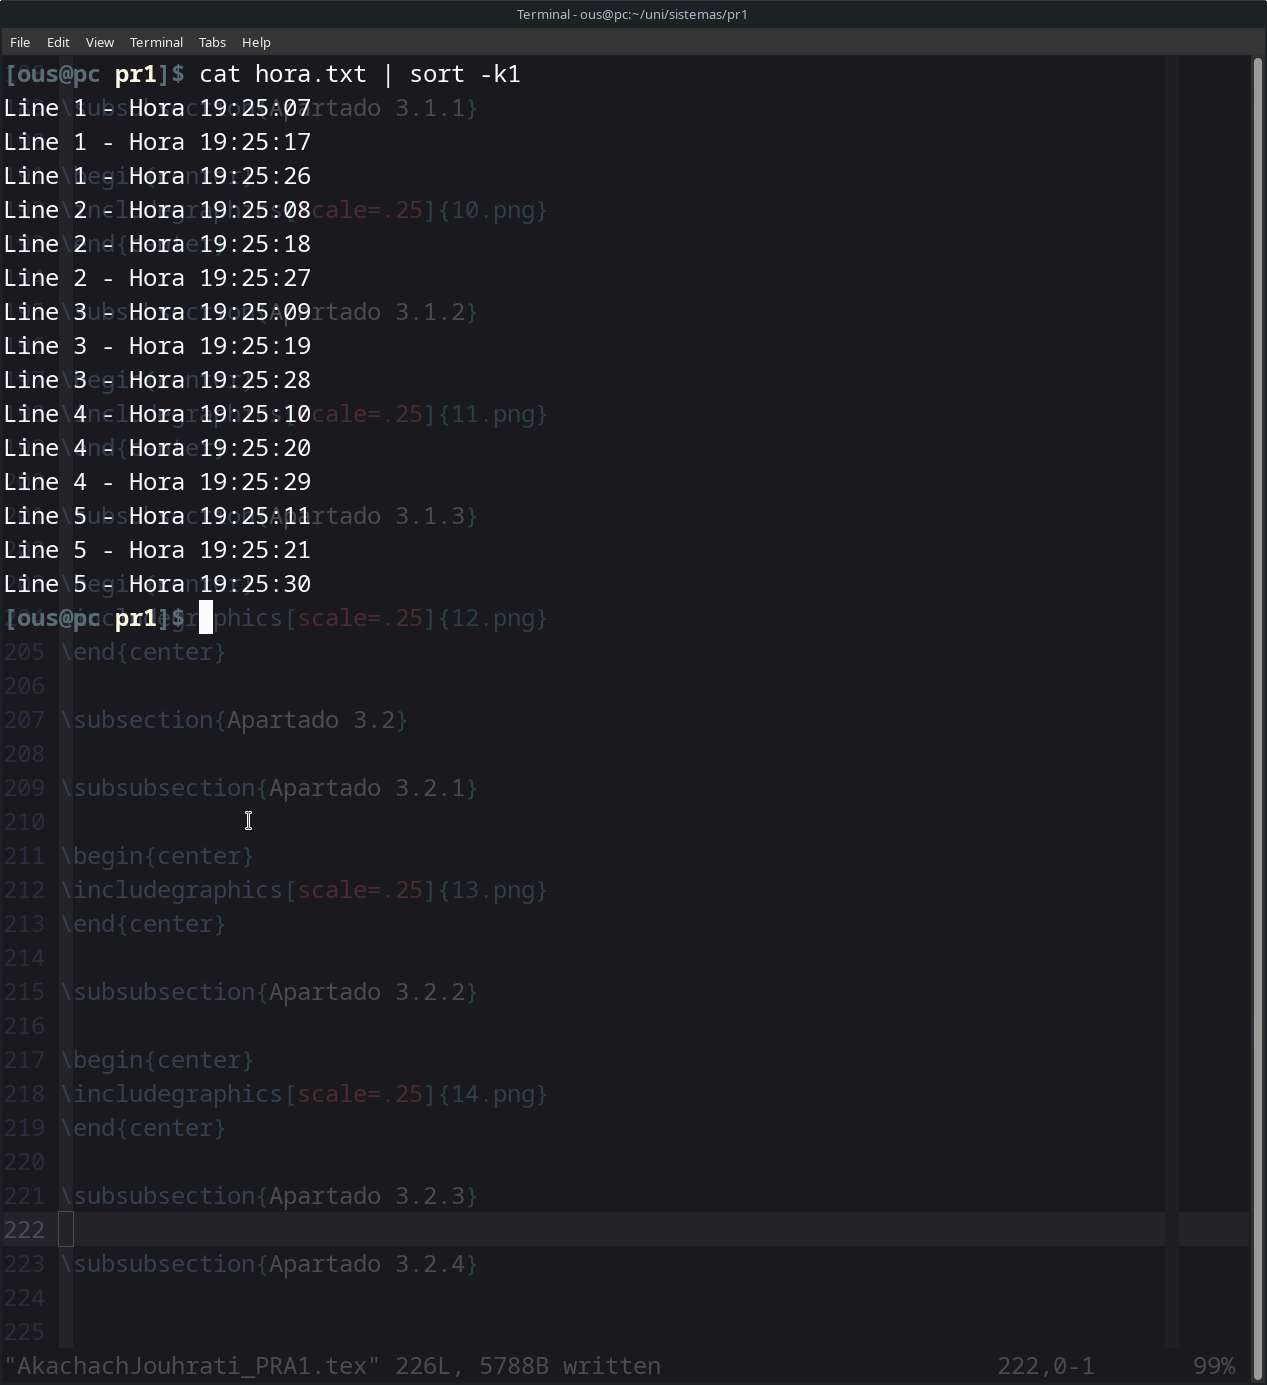
\includegraphics[scale=.25]{../img/15.png}
\end{center}

\newpage

\subsubsection{Apartado 3.2.4}

\begin{center}
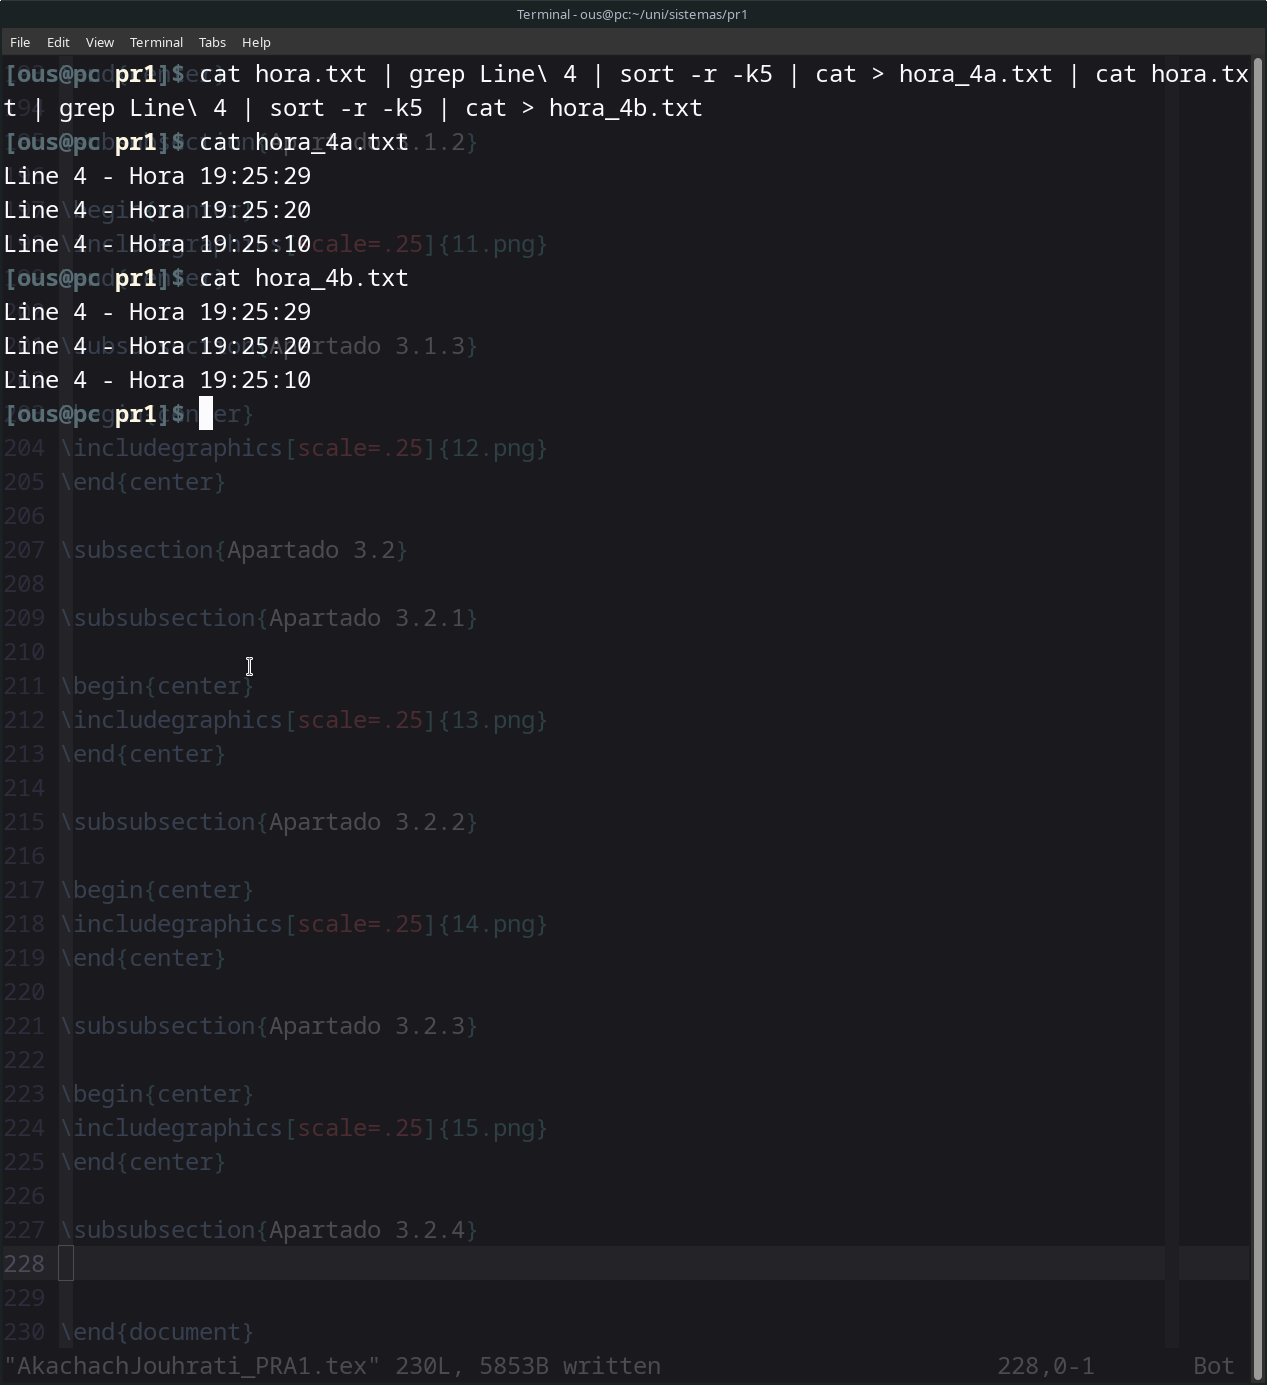
\includegraphics[scale=.25]{../img/16.png}
\end{center}

\end{document}
